\section{System Design} \label{sec:sb-design}

\begin{figure}[t]
  \centering
   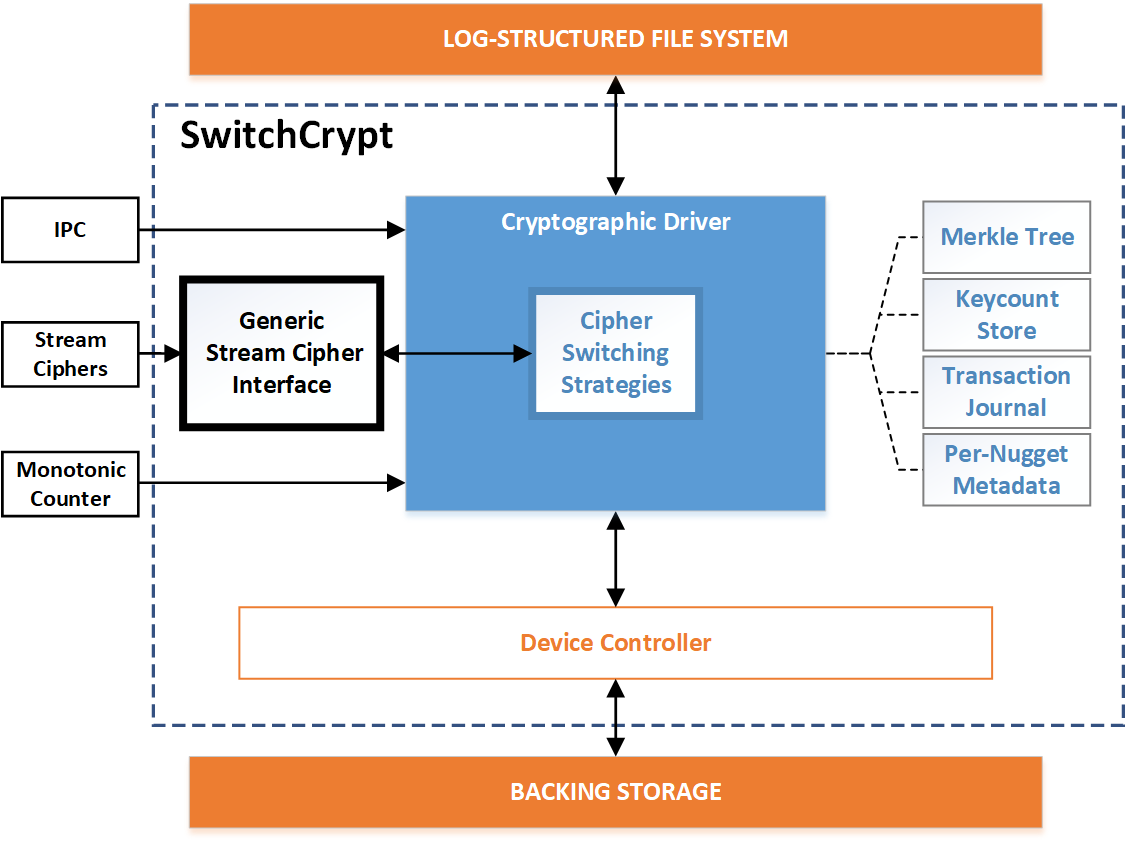
\includegraphics[width=0.8\linewidth]{figs/sb/overview.png}
    \caption{Overview of the StrongBox construction.} \label{fig:sb-overview}
 \end{figure}

StrongBox acts as a translation layer sitting between the drive and the
operating system. It provides confidentiality and integrity guarantees while
minimizing performance loss due to metadata management overhead. StrongBox
accomplishes this by leveraging the speed of stream ciphers over the AES block
cipher and taking advantage of the append-mostly nature of Log-structured
Filesystems (LFS) and modern Flash Translation Layers (FTL)~\cite{SSD}.

Hence, there are several locations where StrongBox could be implemented in the
system stack. StrongBox could be integrated into an LFS kernel module
itself---\eg F2FS---specifically leveraging the flexibility of the Virtual
Filesystem Switch (VFS). StrongBox could be implemented as an actual block
device, or virtual block device layered atop a physical block device; the latter
is where we chose to implement our prototype. StrongBox could even be
implemented within the SSD drive controller's FTL, which handles scatter gather,
garbage collection, wear-leveling, etc.

\figref{sb-overview} illustrates StrongBox's design. StrongBox's metadata is
encapsulated in four components: an in-memory \emph{Merkle Tree} and two
drive-backed byte arrays---the \emph{Keycount Store} and the \emph{Transaction
Journal}---and a persistent monotonic counter we implement with the \emph{Replay
Protected Memory Block} or RPMB. All four are integrated into the
\emph{Cryptographic Driver}, which handles data encryption, verification, and
decryption during interactions with the underlying backing store. These
interactions take place while fulfilling high-level I/O requests received from
the LFS. The \emph{Device Controller} handles low-level I/O between
StrongBox and the backing store.

The rest of this section describes the components referenced in
\figref{sb-overview}. Specifically: we first describe the backing store and
StrongBox's layout for data and metadata. This is followed by an exploration of
the cryptographic driver and how it interacts with that metadata, the role of
the device controller, an overview of rekeying in the backing store, and further
considerations to ensure confidentiality in the case of rollbacks and related
attacks.

\subsection{Backing Store Function and Layout}

The backing store is the storage media on which StrongBox operates.
\figref{sb-backstore} illustrates StrongBox's layout on this store.

\begin{figure}[t]
 \centering
  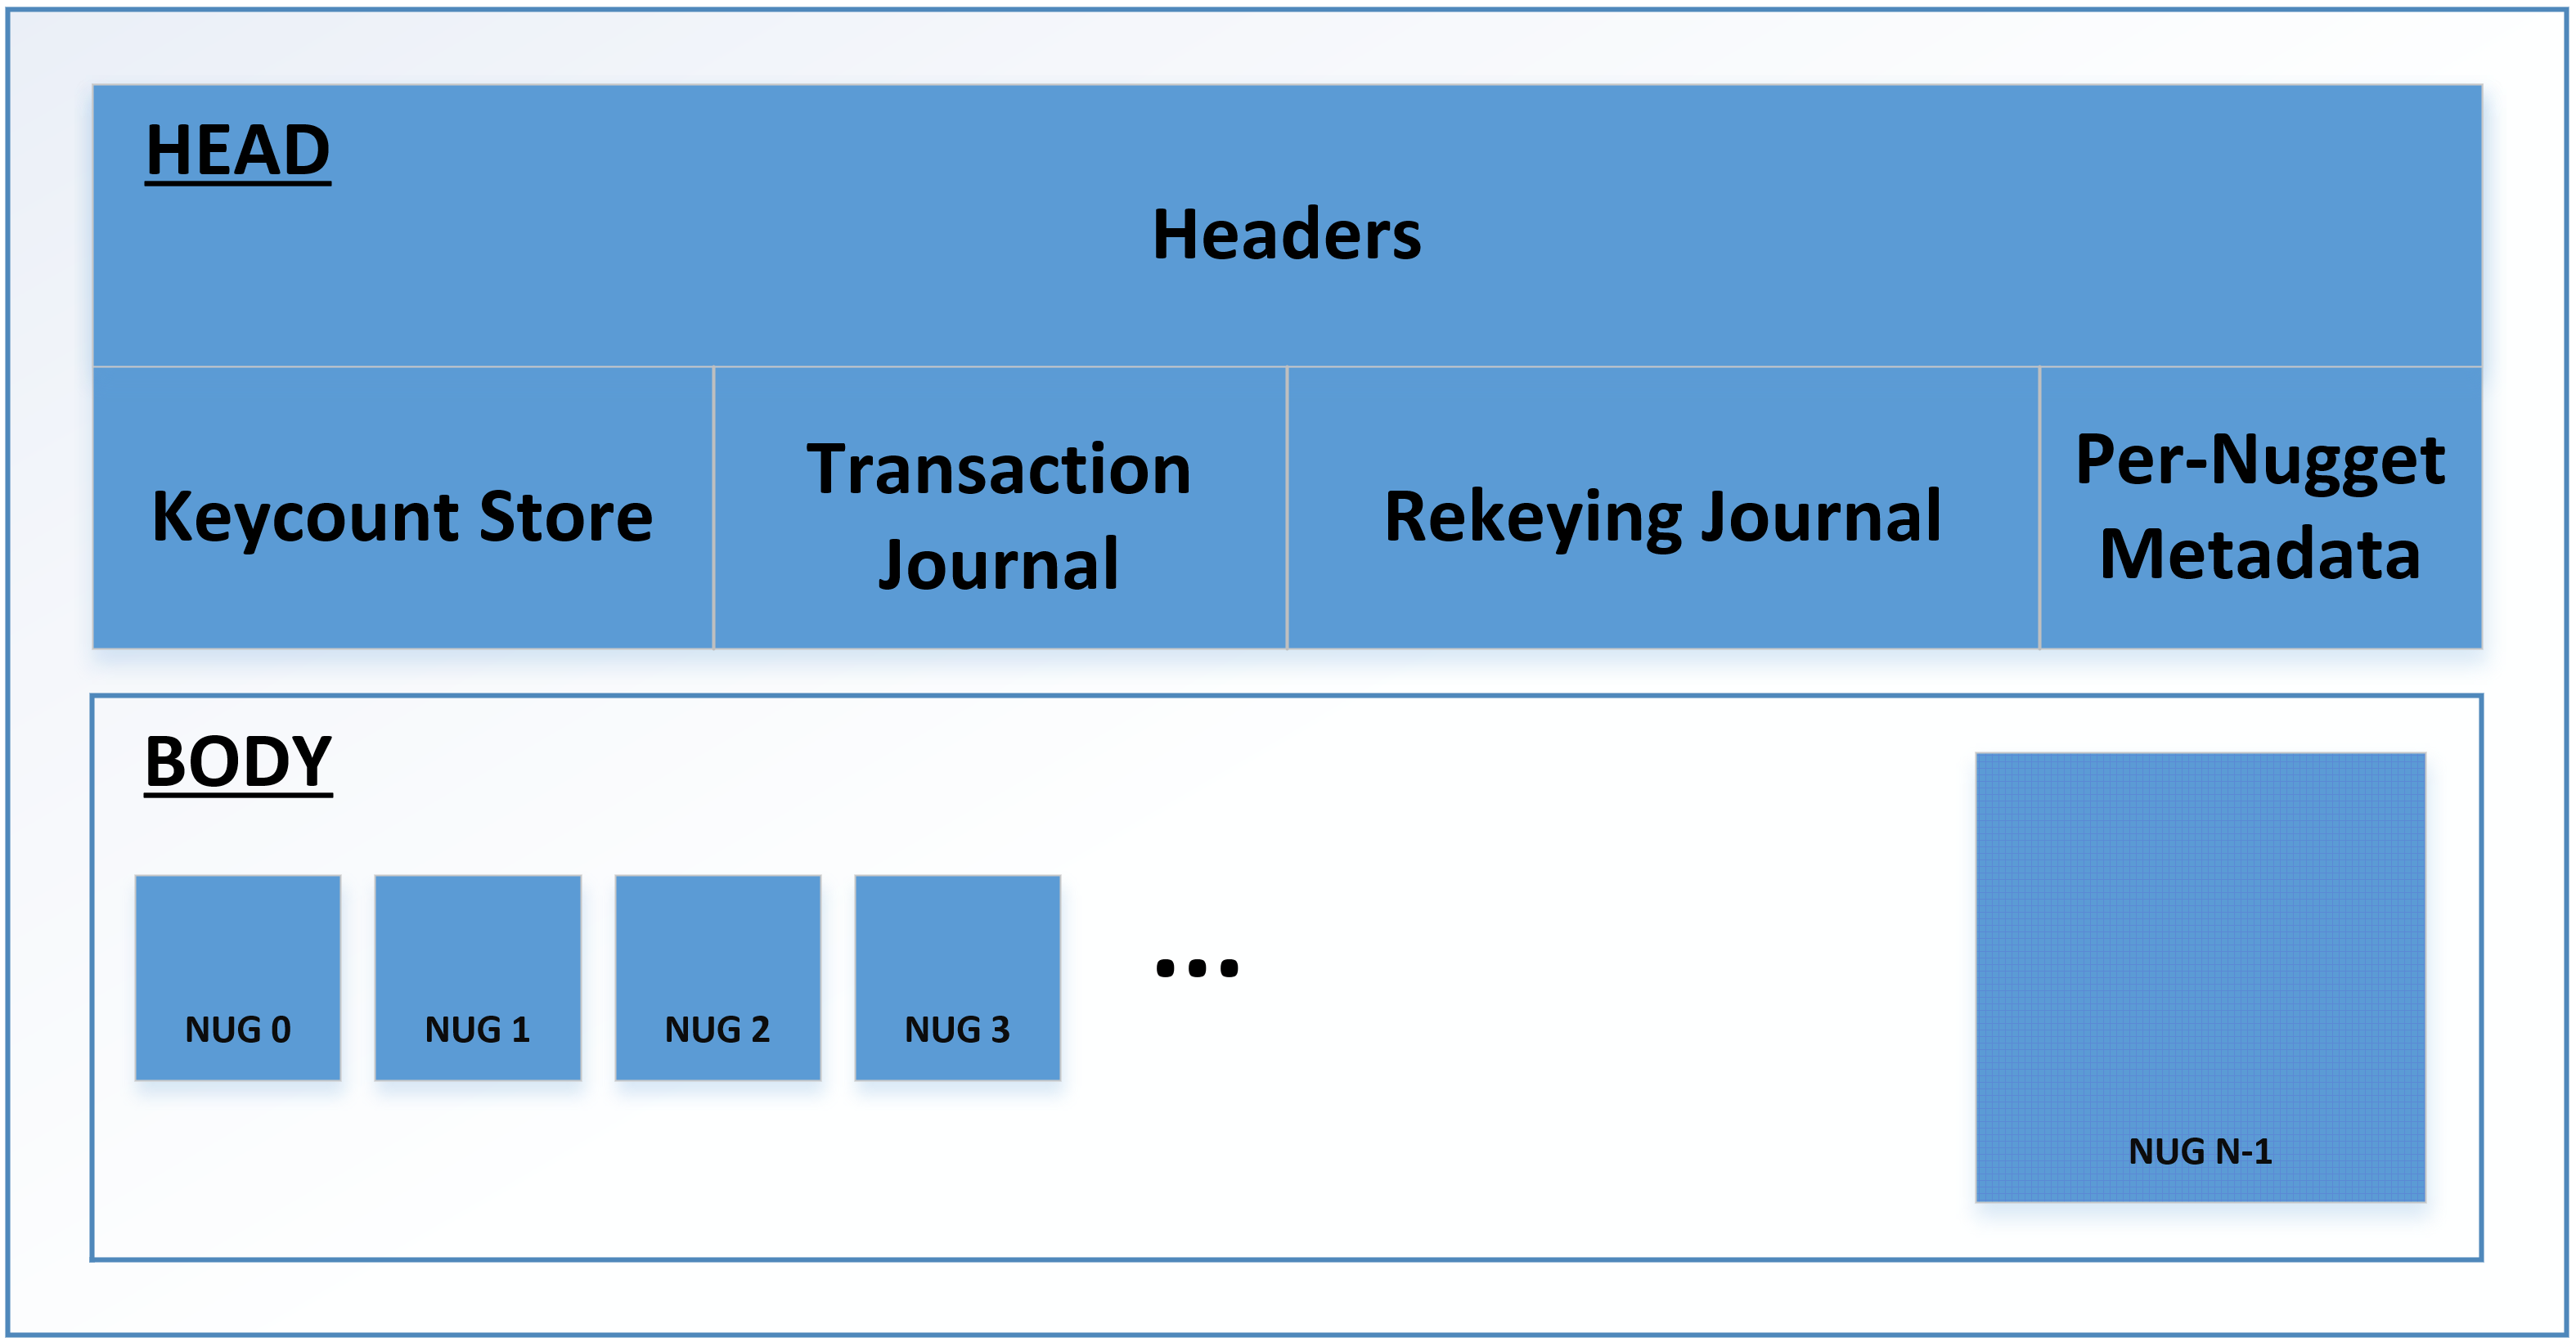
\includegraphics[width=0.8\linewidth]{figs/sb/backstore.png}
   \caption{Layout of StrongBox's backing storage.} \label{fig:sb-backstore}
\end{figure}

In the \textit{body} section of the backing store layout, end-user data is
partitioned into a series of same-size \emph{logical blocks}. These are distinct
from the concept of \emph{physical drive blocks}, which are collections of one
or more drive sectors. To make this distinction clear, we refer to these wider
logical blocks as \emph{nuggets}, marked \textit{NUG} in the Body section of
\figref{sb-backstore}. Hence, a nugget consists of one or more physical drive
blocks, depending on its configured size. Each nugget is subdivided into a
constant number of sub-blocks we refer to as \emph{flakes}.

The reason for these nugget/flake divisions are two-fold:

\begin{enumerate}

\item To track, detect, and handle overwrites and

\item To limit the maximum length of any plaintexts operated on by the
cryptographic driver, decreasing the overhead incurred per I/O operation and per
overwrite.

\end{enumerate}

% Describe how the components in fig 1 are represented on drive and how
% they play into the overall design WITHOUT naming them

Considering the first item, we are required to keep track of writes so that we
may detect when an overwrite occurs. Flakes are key to this tracking. When a
request comes in to write to one or more flakes in a nugget, StrongBox marks the
affected flakes as ``flagged''. Here, ``flagged'' implies that another write to
some portion of that flake would constitute an overwrite. If a new request comes
in to write to one or more of those same flakes another time, StrongBox triggers
a ``rekeying'' procedure over the entire nugget to safely overwrite the old data
in those flakes. This rekeying procedure is necessarily time consuming,
ballooning the overhead of overwrites translated by StrongBox.

Considering the second item, nugget size here governs the granularity of
rekeying while flake size governs granularity when identifying overwrites. A
larger nugget size will increase the penalty incurred with rekeying (you are
re-encrypting a larger number of bytes) while a smaller nugget size will increase
the quantity of nuggets needing to be rekeyed when an overwrite is detected as
well as increase the amount of metadata stored on drive and in memory. On the
other hand, a larger flake size will increase the number of times an incoming
write is seen as an overwrite, with a non-optimal nugget-sized flake requiring a
rekeying on \emph{every write}. A smaller flake size will increase the amount of
metadata stored on drive and in memory.

The size and structure of that metadata is described in greater detail
throughout the rest of this section.

The \textit{head} section of the backing store layout contains the metadata
written to drive during StrongBox's initialization. These headers govern
StrongBox's operation and are, in order:

\begin{enumerate}

\item VERSION, 4 bytes; specifies the StrongBox version originally used to
initialize the backing store

\item SALT, 16 bytes; the salt used in part to derive the global master secret

\item MTRH, 32 bytes; the hash of the Merkle Tree root

\item TPMGLOBALVER, 8 bytes; the monotonic global version count, parity in
hardware-supported secure storage

\item VERIFICATION, 32 bytes; used to determine if the key derived from a
password is correct

\item NUMNUGGETS, 4 bytes; the number of nuggets contained by the backing
store

\item FLAKESPERNUGGET, 4 bytes; the number of flakes/nugget

\item FLAKESIZE, 4 bytes; the size of each flake, in bytes

\item INITIALIZED, 1 byte; used to determine if the backing store has been
properly initialized

\item REKEYING, 4 bytes; the index of the nugget in need of rekeying if there
is a pending rekeying procedure

\end{enumerate}

After the headers, two byte arrays are stored in the Head section: one
of $N$ 8-byte integer \textit{keycounts} and one of $N$ $\ceil{P /
  8}$-byte \textit{transaction journal entries}, where $N$ is the
number of nuggets and $P$ is the number of flakes per nugget.

Finally, the \emph{Rekeying Journal} is stored at the end of the Head section.
The rekeying journal is where nuggets and their associated metadata are
transiently written, enabling StrongBox to resume rekeying in the event that it
is interrupted during the rekeying procedure.

\subsubsection{Metadata-aware Cryptographic Driver}

The cryptographic driver coordinates StrongBox's disparate components.
Its primary function is to map incoming reads and writes to their
proper destinations in the backing store, applying our chosen stream
cipher and message authentication code to encrypt, verify, and decrypt
data on the fly with consideration for metadata management.

When a read request is received, it is first partitioned into affected
nuggets; \eg a read that spans two nuggets is partitioned in half.
For each nugget affected, we calculate which flakes are touched by the
request. We then verify the contents of those flakes. If all the
flakes are valid, whatever subset of data that was requested by the
user is decrypted and returned. \algoref{read} details StrongBox's
read operation.

Like reads, when a write request is received, the request is first
partitioned with respect to affected nuggets. For each affected
nugget, we calculate which flakes are touched by the request and then
check if any of those flakes are marked as flagged in the transaction
journal. If one or more of them have been marked flagged, we trigger
rekeying for this specific nugget (see: \algoref{rekeying}) and end
there. Otherwise, we mark these touched flakes as flagged in the
transaction journal. We then iterate over these touched flakes. For
the first and last flakes touched by the write request, we execute an
internal read request (see: \algoref{read}) to both obtain the flake
data and verify that data with the Merkle Tree. We then overwrite
every touched flake with the data from the requested operation, update
the Merkle Tree to reflect this change, encrypt and write out the new
flake data, and commit all corresponding metadata. \algoref{write}
details StrongBox's write operation.

\begin{algorithm}[t]
%\floatname{algorithm}{Algorithm}
\caption{StrongBox handling an incoming read request.} \label{algo:read}
{\footnotesize 
\begin{algorithmic}[1]
\Require The read request is over a contiguous segment of the backing
store
\Require $\ell, \ell' \leftarrow$ read requested length
\Require $\aleph \leftarrow$ master secret
\Require $n_{index} \leftarrow$ first nugget index to be read
\State $data \leftarrow$ \emph{empty}
\While{$\ell \neq 0$}
    \State $k_{n_{index}} \leftarrow GenKey_{nugget}(n_{index}, \aleph)$
    \State Fetch nugget keycount $n_{kc}$ from Keycount Store.
    \State Calculate indices touched by request: $f_{first}$, $f_{last}$
    \State $n_{flakedat} \leftarrow ReadFlakes(f_{first},\dots,f_{last})$
    \For{$f_{current} = f_{first}$ \textbf{to} $f_{last}$}
        \State $k_{f_{current}} \leftarrow GenKey_{flake}(k_{n_{index}},
        f_{current}, n_{kc})$
        \State $tag_{f_{current}} \leftarrow GenMac(k_{f_{current}},
        n_{flakedat}[f_{current}])$
        \State Verify $tag_{f_{current}}$ in Merkle Tree.
    \EndFor 
    \LineComment{(\textbf{*}) denotes requested subset of nugget data}
    \State $data \leftarrow data + Decrypt(*n_{flakedat}, k_{n_{index}},
    n_{kc})$
    \State $\ell \leftarrow \ell - \|*n_{flakedat}\|$
    \State $n_{index} \leftarrow n_{index} + 1$
\EndWhile 
\\\Return $data$ \Comment{Fulfill the read request}
\Ensure $\|data\| <= \ell'$ 
\Ensure $\ell = 0$
\vskip -1.5em
\end{algorithmic}
}
\end{algorithm}

\begin{algorithm}[t]
%\floatname{algorithm}
\caption{StrongBox handling an incoming write request.} \label{algo:write}
{\footnotesize 
\begin{algorithmic}[1]
\Require The write request is to a contiguous segment of the backing store
\Require $\ell, \ell' \leftarrow$ write requested length
\Require $\aleph \leftarrow$ master secret
\Require $data \leftarrow$ cleartext data to be written
\Require $n_{index} \leftarrow$ first nugget index to be affected
\State Increment secure counter: by 2 if we recovered from a crash, else 1
\While{$\ell \neq 0$}
    \State Calculate indices touched by request: $f_{first}$, $f_{last}$
    \If{Transaction Journal entries for $f_{first},\dots,f_{last} \neq 0$}
        \State Trigger rekeying procedure (see: \algoref{rekeying}).
        \State \textbf{continue}
    \EndIf 
    \State Set Transaction Journal entries for $f_{first},\dots,f_{last}$ to 1
    \State $k_{n_{index}} \leftarrow GenKey_{nugget}(n_{index}, \aleph)$
    \State Fetch nugget keycount $n_{kc}$ from Keycount Store.
    \For{$f_{current} = f_{first}$ \textbf{to} $f_{last}$}
        \State $n_{flakedat} \leftarrow $ \textit{empty}
        \If{$f_{current} == f_{first} \| f_{current} == f_{last}$}
            \State $n_{flakedat} \leftarrow CryptedRead(\textit{FSIZE}, \aleph,
            n_{index}$@$f_{offset})$
        \EndIf 
        \State $n_{flakedat} \leftarrow Encrypt(n_{flakedat}, k_{n_{index}},
        n_{kc})$
        \State $k_{f_{current}} \leftarrow GenKey_{flake}(k_{n_{index}},
        f_{current}, n_{kc})$
        \State $tag_{f_{current}} \leftarrow GenMac(k_{f_{current}},
        n_{flakedat})$
        \State Update new $tag_{f_{current}}$ in Merkle Tree.
        \State $WriteFlake(f_{current}, n_{flakedat})$
        \\\LineComment{(\textbf{*}) denotes requested subset of nugget data if
        applicable}
        \State $\ell \leftarrow \ell - \|*n_{flakedat}\|$
    \EndFor 
    \State $n_{index} \leftarrow n_{index} + 1$
\EndWhile 
\State Update and commit metadata and headers
\Ensure $\ell = 0$
\vskip -1.5em
\end{algorithmic}
}
\end{algorithm}

% Algorithmic analysis?

\subsubsection{Transaction Journal}

An overwrite breaks the security guarantee offered by any stream
cipher. To prevent this failure, StrongBox tracks incoming write
requests to prevent overwrites. This tracking is done with the
transaction journal, featured in \figref{sb-overview}.

% Describe how this component meets that need
The transaction journal consists of $N$ $\ceil{P / 8}$-byte bit
vectors where $N$ is the number of nuggets and $P$ is the number of
flakes per nugget. A bit vector $v$ contains at least $P$ bits $v = \{
b_0, b_1, b_2, \dots, b_{P-1}, \dots \}$, with extra bits ignored.
Each vector is associated with a nugget and each bit with a flake
belonging to that nugget. When an incoming write request occurs, the
corresponding bit vector is updated (set to 1) to reflect the new
flagged state of those flakes.

% Describe briefly TJ's relation to writes: when it's referenced and when it's
% changed
The transaction journal is referenced during each write request, where
it is updated to reflect the state of the nugget and checked to ensure
the operation does not constitute an overwrite. If the operation
\textit{does} constitute an overwrite, StrongBox triggers a rekeying
procedure for the entire nugget before safely completing the request.

\subsubsection{Merkle Tree} \label{sec:merkle}

Tracking writes with the transaction journal may stymie a passive
attacker by preventing explicit overwrites, but a sufficiently
motivated active attacker could resort to all manner of cut-and-paste
tactics with nuggets, flakes, and even blocks and sectors. If, for
example, an attacker purposefully zeroed-out the transaction journal
entry pertaining to a specific nugget in some out-of-band
manner---such as when StrongBox is shut down and then later
re-initialized with the same backing store---StrongBox would consider
any successive incoming writes as if the nugget were in a completely
clean state, even though it actually is not. This attack would force
StrongBox to make compromising overwrites. To prevent such attacks, we
must ensure that the backing store is always in a valid state. More
concretely: we must provide an integrity guarantee on top of a
confidentiality guarantee.

StrongBox uses our chosen Message Authentication Code (MAC) generating algorithm
and each flake's unique key to generate a per-flake MAC tag (``MACed''). The
purpose of this tag is to authenticate flake data and confirm that it has not
been tampered with. Each tag is then appended to the Merkle Tree along with
StrongBox's metadata.

The transaction journal entries are handled specially in that the bit
vectors are MACed and the result is appended to the Merkle Tree. This is done to
save space.

The Merkle Tree then ties the integrity of any single flake to the integrity of
the system as a whole such that if the former fails, \ie{there is a MAC tag
mismatch for any particular flake}, the latter immediately and obviously fails.

\subsubsection{Keycount Store}

To prevent a many-time pad attack, each nugget is assigned its own
form of nonce we refer to as a \emph{keycount}. The keycount store in
\figref{sb-overview} represents a byte-array containing $N$ 8-byte
integer keycounts indexed to each nugget. Along with acting as the
per-nugget nonce consumed by the stream cipher, the keycount is used
to derive the per-flake unique subkeys used in MAC tag generation.

\subsection{Rekeying Procedure}

When a write request would constitute an overwrite, StrongBox will
trigger a rekeying process instead of executing the write normally.
This rekeying process allows the write to proceed without causing a
catastrophic confidentiality violation.

When rekeying begins, the nugget in question is loaded into memory and
decrypted. The target data is written into its proper offset in this decrypted
nugget. The nugget is then encrypted, this time with a different nonce
(\textit{keycount + 1}), and written to the backing store, replacing the
outdated nugget data. See: \algoref{rekeying}.

\begin{algorithm}[t]
%\floatname{algorithm}
\caption{StrongBox rekeying process.} \label{algo:rekeying}
{\footnotesize 
\begin{algorithmic}[1]
\Require The original write applied to a contiguous backing store segment
\Require $\ell \leftarrow$ write requested length
\Require $\aleph \leftarrow$ master secret
\Require $data \leftarrow$ cleartext data to be written
\Require $n_{index} \leftarrow$ nugget rekeying target

\Comment{Read in and decrypt the entire nugget}
\State $n_{nuggetdat} \leftarrow CryptedRead(\textit{NSIZE}, \aleph, n_{index})$
\State Calculate indices touched by request: $f_{first}$, $f_{last}$
\State Write $data$ into $n_{nuggetdat}$ at proper offset with length $\ell$
\State Set Transaction Journal entries for $f_{first},\dots,f_{last}$ to 1
\State $k_{n_{index}} \leftarrow GenKey_{nugget}(n_{index}, \aleph)$
\State Fetch nugget keycount $n_{kc}$ from Keycount Store. Increment it by one.
\State $n_{nuggetdat} \leftarrow Encrypt(n_{nuggetdat}, k_{n_{index}}, n_{kc})$
\State Commit $n_{nuggetdat}$ to the backing store

\Comment{Iterate over all flakes in the nugget}
\ForAll{flakes $f_{current}$ \textbf{in} $n_{index}$}
    \State $k_{f_{current}} \leftarrow GenKey_{flake}(k_{n_{index}},
    f_{current}, n_{kc})$
    \State Copy $f_{current}$ data from $n_{nuggetdat} \rightarrow n_{flakedat}$
    \State $tag_{f_{current}} \leftarrow GenMac(k_{f_{current}}, n_{flakedat})$
    \State Update new $tag_{f_{current}}$ in Merkle Tree.
\EndFor 
\State Update and commit metadata and headers
\vskip -1.5em
\end{algorithmic}
}
\end{algorithm}

\subsection{Defending Against Rollback Attacks}

To prevent StrongBox from making overwrites, the status of each flake
is tracked and overwrites trigger a rekeying procedure. Tracking flake
status alone is not enough, however. An attacker could take a snapshot
of the backing store in its current state and then easily rollback to
a previously valid state. At this point, the attacker could have
StrongBox make writes that it does not recognize as overwrites.

With AES-XTS, the threat posed by rolling the backing store to a
previously valid state is outside of its threat model. Despite this,
data confidentiality guaranteed by AES-XTS holds in the event of a
rollback, even if integrity is violated.

StrongBox uses a monotonic global version counter to detect rollbacks.
When a rollback is detected, StrongBox will refuse to initialize
unless forced, using root permission. Whenever a write request is
completed, this global version counter is committed to the backing
store, committed to secure hardware, and updated in the in-memory
Merkle Tree.

\subsection{Recovering from Inconsistent State}

If StrongBox is interrupted during operation, the backing store---consisting of
user data and StrongBox metadata---will be left in an inconsistent state.
StrongBox relies on the overlying filesystem \eg{F2FS} to manage user-data
recovery, which is what these filesystems are designed to do and do well. We
detail how StrongBox handles its own inconsistent metadata.

Let $c$ be the value of the on-chip monotonic global version counter and $d$ be
the value of the on-drive global version counter header (TPMGLOBALVER). Consider
the following:

\begin{itemize}

\item \emph{$c == d$ and MTRH is consistent:} StrongBox is operating
  normally and will mount without issue.

\item \emph{$c<d$ or $c == d$ but MTRH is inconsistent:} Since the
  global version counter is updated before any write, this case cannot
  be reached unless the backing store was manipulated by an attacker.
  So, StrongBox will refuse to initialize and cannot be force mounted.

\item \emph{$c > d + 1$:} Since the global version counter is updated
  once per write, this case cannot be reached unless the backing store
  was rolled back or otherwise manipulated by an attacker. In this
  case, the root user is warned and StrongBox will refuse to
  initialize and cannot be force mounted unless the MTRH is
  consistent. We allow the root user to force mount here if the root
  user initiated the rollback themselves, such as when recovering from
  a drive backup.

\item \emph{$c == d + 1$:} In this case, StrongBox likely crashed
  during a write, perhaps during an attempted rekeying. If the
  rekeying journal is empty or the system cannot complete the rekeying
  and/or bring the MTRH into a consistent state, the root user is
  warned and allowed to force mount. Otherwise, StrongBox will not
  initialize.

\end{itemize}

For subsequent rekeying efforts in the latter two cases, rather than
incrementing the corresponding keystore counters by 1 during rekeying,
they will be incremented by 2. This is done to prevent potential reuse
of any derived nugget keys that might have been in use right before
StrongBox crashed.

When StrongBox can detect tampering, it will not initialize. When StrongBox
cannot distinguish between tampering and crash, it offers the root user a choice
to force mount. Thus, an attacker could force a crash and use root access to
force mount. We assume, however, that if an attacker has root access to a
device, its security is already compromised.
